\documentclass[11pt,preprint, authoryear]{elsarticle}

\usepackage{lmodern}
%%%% My spacing
\usepackage{setspace}
\setstretch{1.2}
\DeclareMathSizes{12}{14}{10}{10}

% Wrap around which gives all figures included the [H] command, or places it "here". This can be tedious to code in Rmarkdown.
\usepackage{float}
\let\origfigure\figure
\let\endorigfigure\endfigure
\renewenvironment{figure}[1][2] {
    \expandafter\origfigure\expandafter[H]
} {
    \endorigfigure
}

\let\origtable\table
\let\endorigtable\endtable
\renewenvironment{table}[1][2] {
    \expandafter\origtable\expandafter[H]
} {
    \endorigtable
}


\usepackage{ifxetex,ifluatex}
\usepackage{fixltx2e} % provides \textsubscript
\ifnum 0\ifxetex 1\fi\ifluatex 1\fi=0 % if pdftex
  \usepackage[T1]{fontenc}
  \usepackage[utf8]{inputenc}
\else % if luatex or xelatex
  \ifxetex
    \usepackage{mathspec}
    \usepackage{xltxtra,xunicode}
  \else
    \usepackage{fontspec}
  \fi
  \defaultfontfeatures{Mapping=tex-text,Scale=MatchLowercase}
  \newcommand{\euro}{€}
\fi

\usepackage{amssymb, amsmath, amsthm, amsfonts}

\def\bibsection{\section*{References}} %%% Make "References" appear before bibliography


\usepackage[round]{natbib}

\usepackage{longtable}
\usepackage[margin=2.3cm,bottom=2cm,top=2.5cm, includefoot]{geometry}
\usepackage{fancyhdr}
\usepackage[bottom, hang, flushmargin]{footmisc}
\usepackage{graphicx}
\numberwithin{equation}{section}
\numberwithin{figure}{section}
\numberwithin{table}{section}
\setlength{\parindent}{0cm}
\setlength{\parskip}{1.3ex plus 0.5ex minus 0.3ex}
\usepackage{textcomp}
\renewcommand{\headrulewidth}{0.2pt}
\renewcommand{\footrulewidth}{0.3pt}

\usepackage{array}
\newcolumntype{x}[1]{>{\centering\arraybackslash\hspace{0pt}}p{#1}}

%%%%  Remove the "preprint submitted to" part. Don't worry about this either, it just looks better without it:
\makeatletter
\def\ps@pprintTitle{%
  \let\@oddhead\@empty
  \let\@evenhead\@empty
  \let\@oddfoot\@empty
  \let\@evenfoot\@oddfoot
}
\makeatother

 \def\tightlist{} % This allows for subbullets!

\usepackage{hyperref}
\hypersetup{breaklinks=true,
            bookmarks=true,
            colorlinks=true,
            citecolor=blue,
            urlcolor=blue,
            linkcolor=blue,
            pdfborder={0 0 0}}


% The following packages allow huxtable to work:
\usepackage{siunitx}
\usepackage{multirow}
\usepackage{hhline}
\usepackage{calc}
\usepackage{tabularx}
\usepackage{booktabs}
\usepackage{caption}


\newenvironment{columns}[1][]{}{}

\newenvironment{column}[1]{\begin{minipage}{#1}\ignorespaces}{%
\end{minipage}
\ifhmode\unskip\fi
\aftergroup\useignorespacesandallpars}

\def\useignorespacesandallpars#1\ignorespaces\fi{%
#1\fi\ignorespacesandallpars}

\makeatletter
\def\ignorespacesandallpars{%
  \@ifnextchar\par
    {\expandafter\ignorespacesandallpars\@gobble}%
    {}%
}
\makeatother

\newlength{\cslhangindent}
\setlength{\cslhangindent}{1.5em}
\newenvironment{CSLReferences}%
  {\setlength{\parindent}{0pt}%
  \everypar{\setlength{\hangindent}{\cslhangindent}}\ignorespaces}%
  {\par}


\urlstyle{same}  % don't use monospace font for urls
\setlength{\parindent}{0pt}
\setlength{\parskip}{6pt plus 2pt minus 1pt}
\setlength{\emergencystretch}{3em}  % prevent overfull lines
\setcounter{secnumdepth}{5}

%%% Use protect on footnotes to avoid problems with footnotes in titles
\let\rmarkdownfootnote\footnote%
\def\footnote{\protect\rmarkdownfootnote}
\IfFileExists{upquote.sty}{\usepackage{upquote}}{}

%%% Include extra packages specified by user

%%% Hard setting column skips for reports - this ensures greater consistency and control over the length settings in the document.
%% page layout
%% paragraphs
\setlength{\baselineskip}{12pt plus 0pt minus 0pt}
\setlength{\parskip}{12pt plus 0pt minus 0pt}
\setlength{\parindent}{0pt plus 0pt minus 0pt}
%% floats
\setlength{\floatsep}{12pt plus 0 pt minus 0pt}
\setlength{\textfloatsep}{20pt plus 0pt minus 0pt}
\setlength{\intextsep}{14pt plus 0pt minus 0pt}
\setlength{\dbltextfloatsep}{20pt plus 0pt minus 0pt}
\setlength{\dblfloatsep}{14pt plus 0pt minus 0pt}
%% maths
\setlength{\abovedisplayskip}{12pt plus 0pt minus 0pt}
\setlength{\belowdisplayskip}{12pt plus 0pt minus 0pt}
%% lists
\setlength{\topsep}{10pt plus 0pt minus 0pt}
\setlength{\partopsep}{3pt plus 0pt minus 0pt}
\setlength{\itemsep}{5pt plus 0pt minus 0pt}
\setlength{\labelsep}{8mm plus 0mm minus 0mm}
\setlength{\parsep}{\the\parskip}
\setlength{\listparindent}{\the\parindent}
%% verbatim
\setlength{\fboxsep}{5pt plus 0pt minus 0pt}



\begin{document}



\begin{frontmatter}  %

\title{Data Science: Machine Learning}

% Set to FALSE if wanting to remove title (for submission)




\author[Add1]{Samantha Scott}
\ead{20945043@sun.ac.za}





\address[Add1]{Stellenbosch University, Cape Town, South Africa}



\vspace{1cm}


\begin{keyword}
\footnotesize{
Machine Learning \sep Heart Disease Prediction \sep Random Forests \\
\vspace{0.3cm}
}
\end{keyword}



\vspace{0.5cm}

\end{frontmatter}


\newpage
\renewcommand{\contentsname}{Table of Contents}
{\tableofcontents}
\newpage

%________________________
% Header and Footers
%%%%%%%%%%%%%%%%%%%%%%%%%%%%%%%%%
\pagestyle{fancy}
\chead{}
\rhead{Predicting Heart Disease}
\lfoot{}
\rfoot{\footnotesize Page \thepage}
\lhead{}
%\rfoot{\footnotesize Page \thepage } % "e.g. Page 2"
\cfoot{}

%\setlength\headheight{30pt}
%%%%%%%%%%%%%%%%%%%%%%%%%%%%%%%%%
%________________________

\headsep 35pt % So that header does not go over title




\hypertarget{introduction}{%
\section{Introduction}\label{introduction}}

The following paper is a comparison between two Machine Learning
algorithms, namely Random Forests and Support Vector Machines, as
prediction tools. Using a Linear Regression model as a baseline, the
RMSE scores are compared.

\hypertarget{research-question}{%
\section{Research Question}\label{research-question}}

Problem type: supervised binomial classification

``Much like EDA, the ML process is very iterative and heurstic-based.
With minimal knowledge of the problem or data at hand, it is difficult
to know which ML method will perform best. This is known as the no free
lunch theorem for ML (Wolpert 1996). Consequently, it is common for many
ML approaches to be applied, evaluated, and modified before a final,
optimal model can be determined. Performing this process correctly
provides great confidence in our outcomes. If not, the results will be
useless and, potentially, damaging.1''

``RMSE: Root mean squared error. This simply takes the square root of
the MSE metric so that your error is in the same units as your response
variable. If your response variable units are dollars, the units of MSE
are dollars-squared, but the RMSE will be in dollars. Objective:
minimize''

\hypertarget{data-and-methodology}{%
\section{Data and Methodology}\label{data-and-methodology}}

The data used in this investigation is heart disease data from Kaggle.

``Support vector machines (SVMs) offer a direct approach to binary
classification: try to find a hyperplane in some feature space that
``best'' separates the two classes. In practice, however, it is
difficult (if not impossible) to find a hyperplane to perfectly separate
the classes using just the original features. SVMs overcome this by
extending the idea of finding a separating hyperplane in two ways: (1)
loosen what we mean by ``perfectly separates'', and (2) use the
so-called kernel trick to enlarge the feature space to the point that
perfect separation of classes is (more) likely.''

\hypertarget{results-and-discussion}{%
\section{Results and Discussion}\label{results-and-discussion}}

\hypertarget{random-forests}{%
\subsection{Random Forests}\label{random-forests}}

\begin{verbatim}
## 
## Call:
##  randomForest(formula = heart_disease_present ~ ., data = train_1,      ntree = 500) 
##                Type of random forest: classification
##                      Number of trees: 500
## No. of variables tried at each split: 3
## 
##         OOB estimate of  error rate: 12.7%
## Confusion matrix:
##    0  1 class.error
## 0 70  6  0.07894737
## 1 10 40  0.20000000
\end{verbatim}

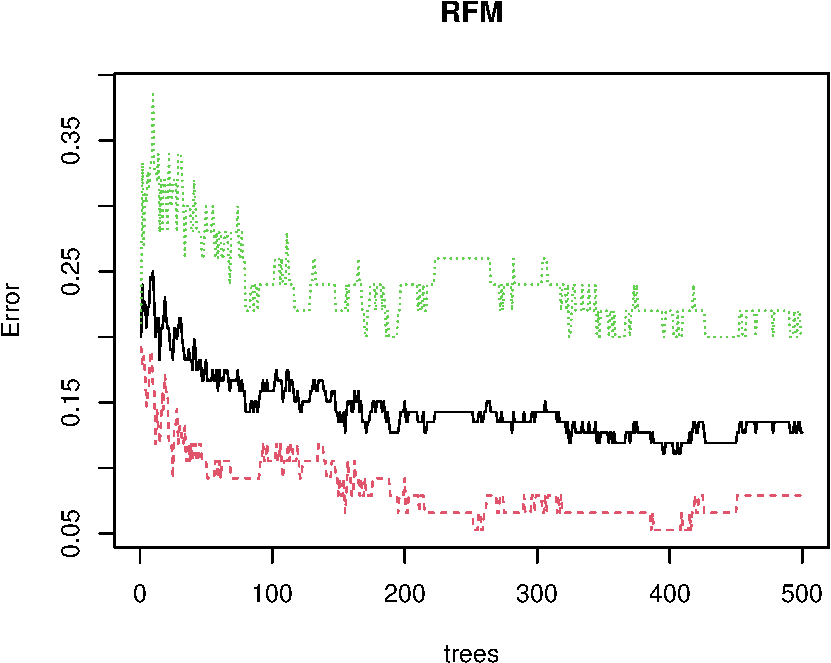
\includegraphics{ML_project_files/figure-latex/unnamed-chunk-5-1.pdf}

\begin{verbatim}
## [1] 3
\end{verbatim}

\begin{verbatim}
## mtry = 3  OOB error = 11.11% 
## Searching left ...
## mtry = 2     OOB error = 9.52% 
## 0.1428571 0.01 
## Searching right ...
## mtry = 4     OOB error = 13.49% 
## -0.4166667 0.01
\end{verbatim}

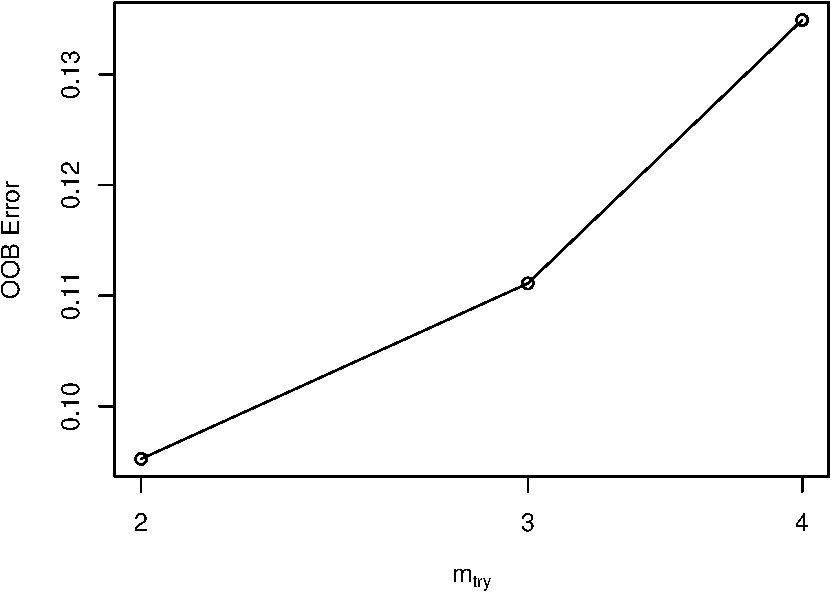
\includegraphics{ML_project_files/figure-latex/unnamed-chunk-7-1.pdf}

\begin{verbatim}
##       mtry  OOBError
## 2.OOB    2 0.0952381
## 3.OOB    3 0.1111111
## 4.OOB    4 0.1349206
\end{verbatim}

\begin{verbatim}
## [1] 2
\end{verbatim}

\begin{verbatim}
## 
## Call:
##  randomForest(formula = heart_disease_present ~ ., data = train_1,      mtry = best.m, ntree = 601, importance = TRUE) 
##                Type of random forest: classification
##                      Number of trees: 601
## No. of variables tried at each split: 2
## 
##         OOB estimate of  error rate: 11.9%
## Confusion matrix:
##    0  1 class.error
## 0 71  5  0.06578947
## 1 10 40  0.20000000
\end{verbatim}

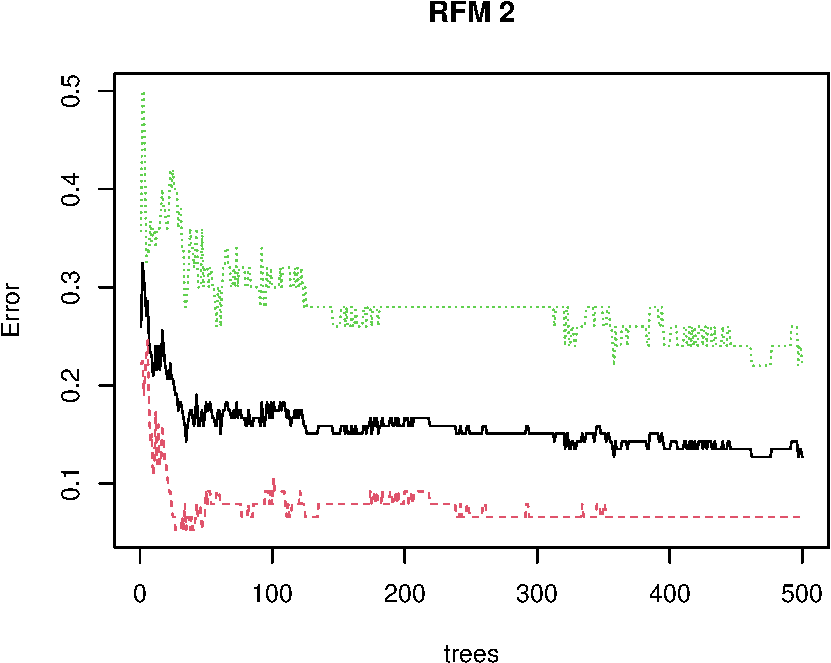
\includegraphics{ML_project_files/figure-latex/unnamed-chunk-10-1.pdf}

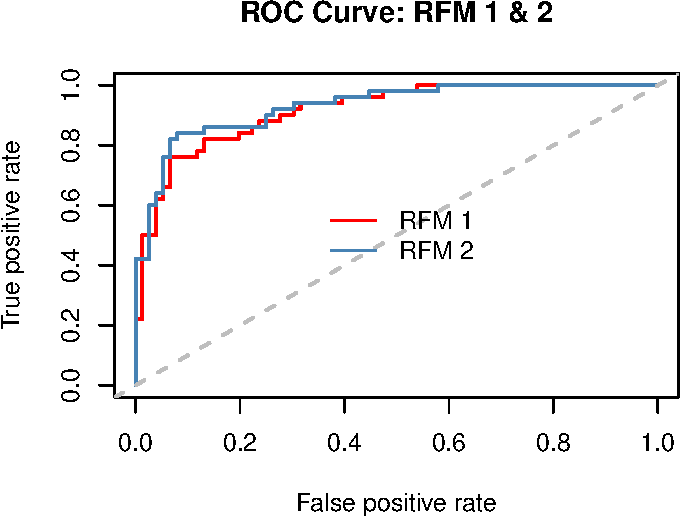
\includegraphics{ML_project_files/figure-latex/unnamed-chunk-12-1.pdf}

\begin{verbatim}
## [1] 0.7407407
\end{verbatim}

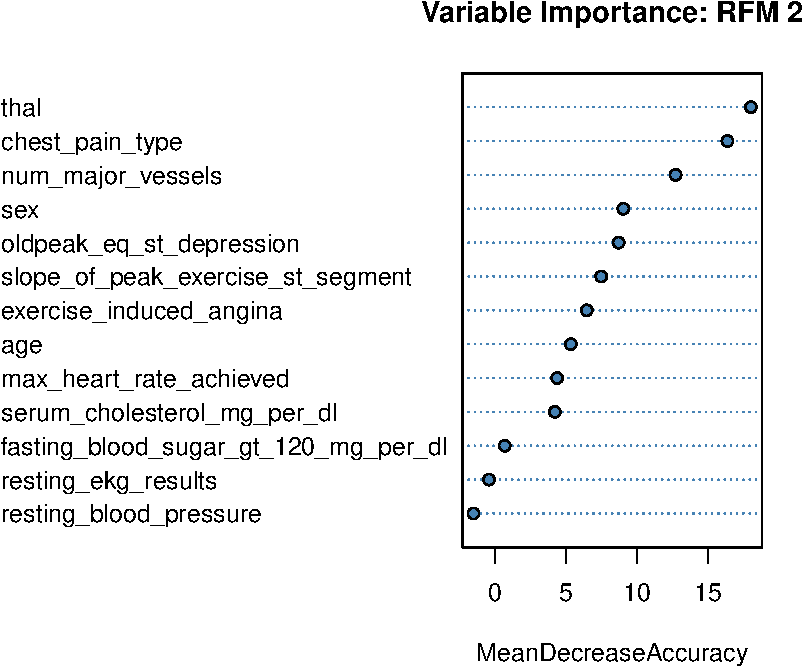
\includegraphics{ML_project_files/figure-latex/unnamed-chunk-15-1.pdf}

\begin{verbatim}
## [1] 0.7407407
\end{verbatim}

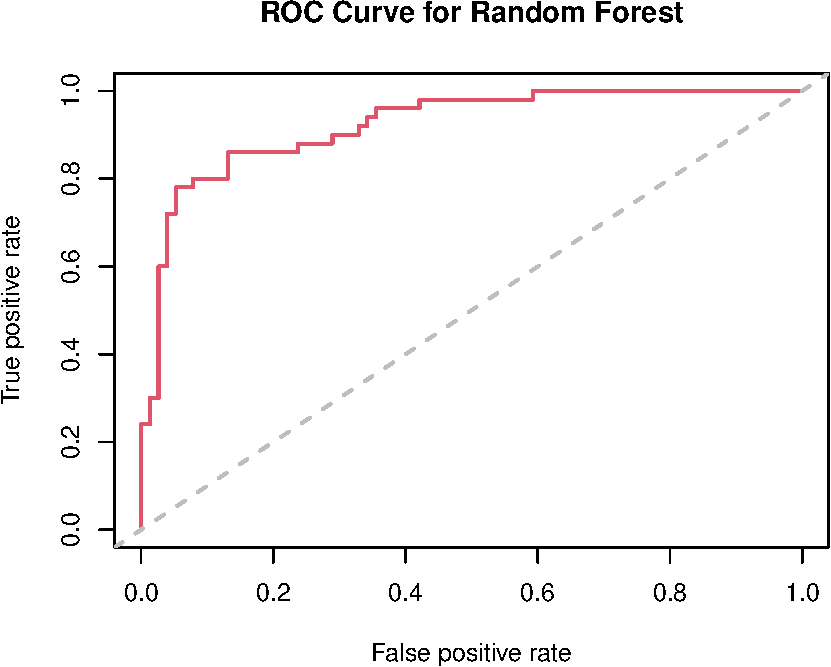
\includegraphics{ML_project_files/figure-latex/unnamed-chunk-17-1.pdf}

\hypertarget{support-vector-machine}{%
\subsection{Support Vector Machine}\label{support-vector-machine}}

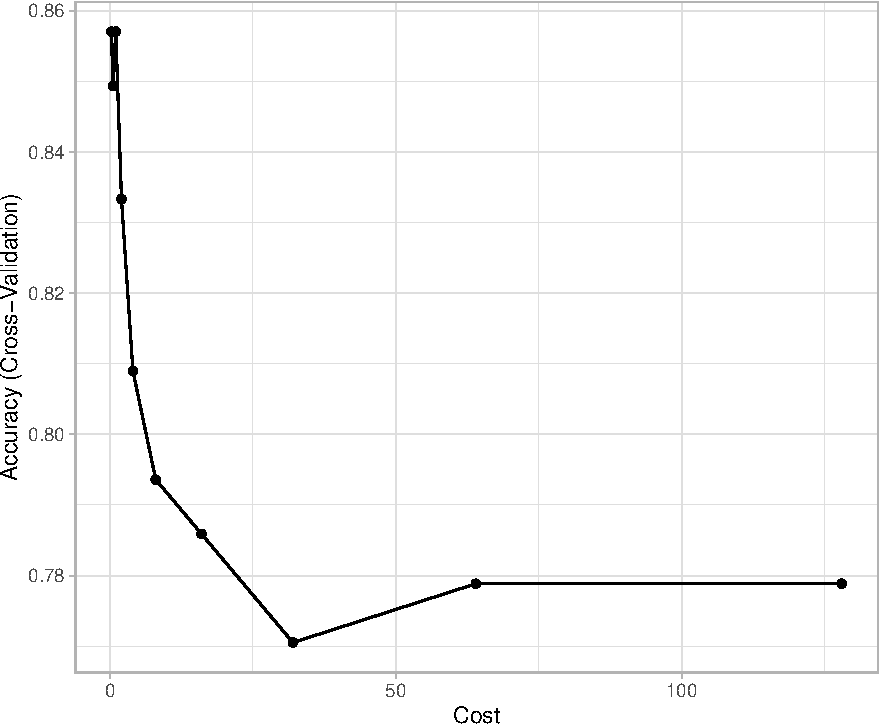
\includegraphics{ML_project_files/figure-latex/unnamed-chunk-19-1.pdf}

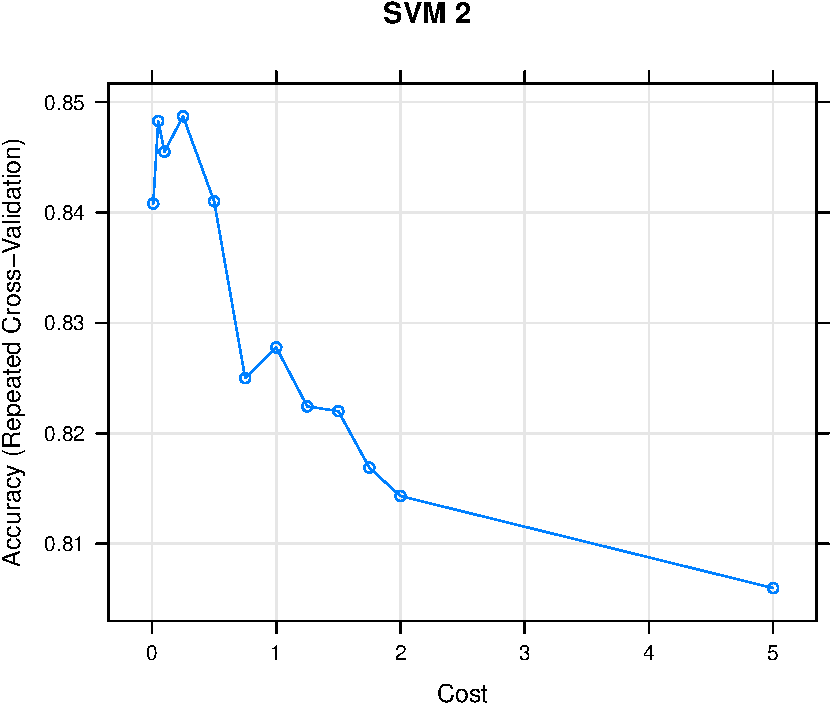
\includegraphics{ML_project_files/figure-latex/unnamed-chunk-21-1.pdf}

\begin{verbatim}
## [1] 0.7777778
\end{verbatim}

\hypertarget{conclusion}{%
\section{Conclusion}\label{conclusion}}

\hypertarget{reference-list}{%
\section{Reference List}\label{reference-list}}

\hypertarget{appendix}{%
\section{Appendix}\label{appendix}}

\begin{verbatim}
## 
##         0         1 
## 0.5555556 0.4444444
\end{verbatim}

\bibliography{Tex/ref}





\end{document}
